\documentclass[../vis.tex]{subfiles}
\begin{document}
\begin{figure*}[h!]
\centering
\subfloat[Voronoi diagram layer]{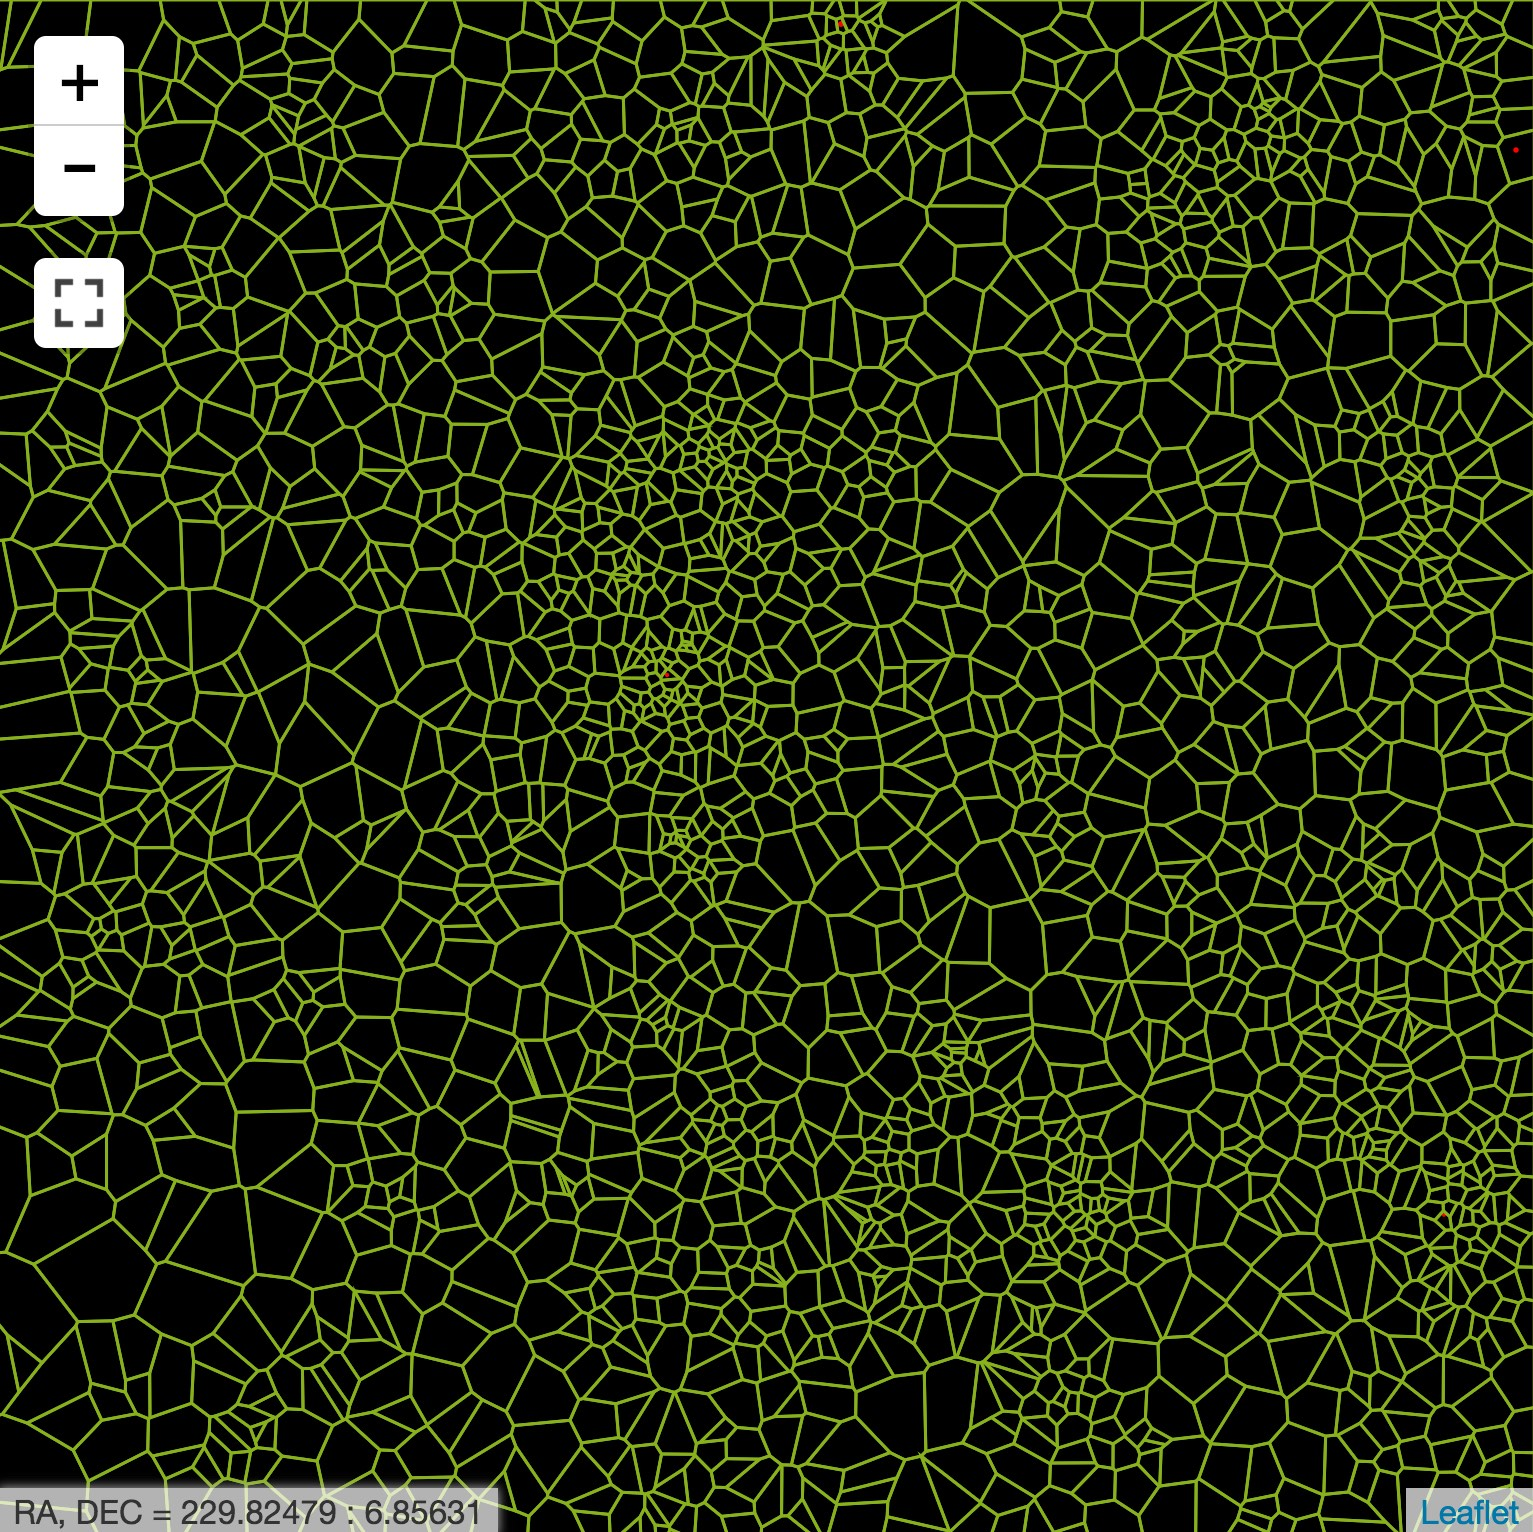
\includegraphics[width=0.4\textwidth]{FIG6a}\label{fig:v_1}}
\quad
\subfloat[Minimum spanning tree layer]{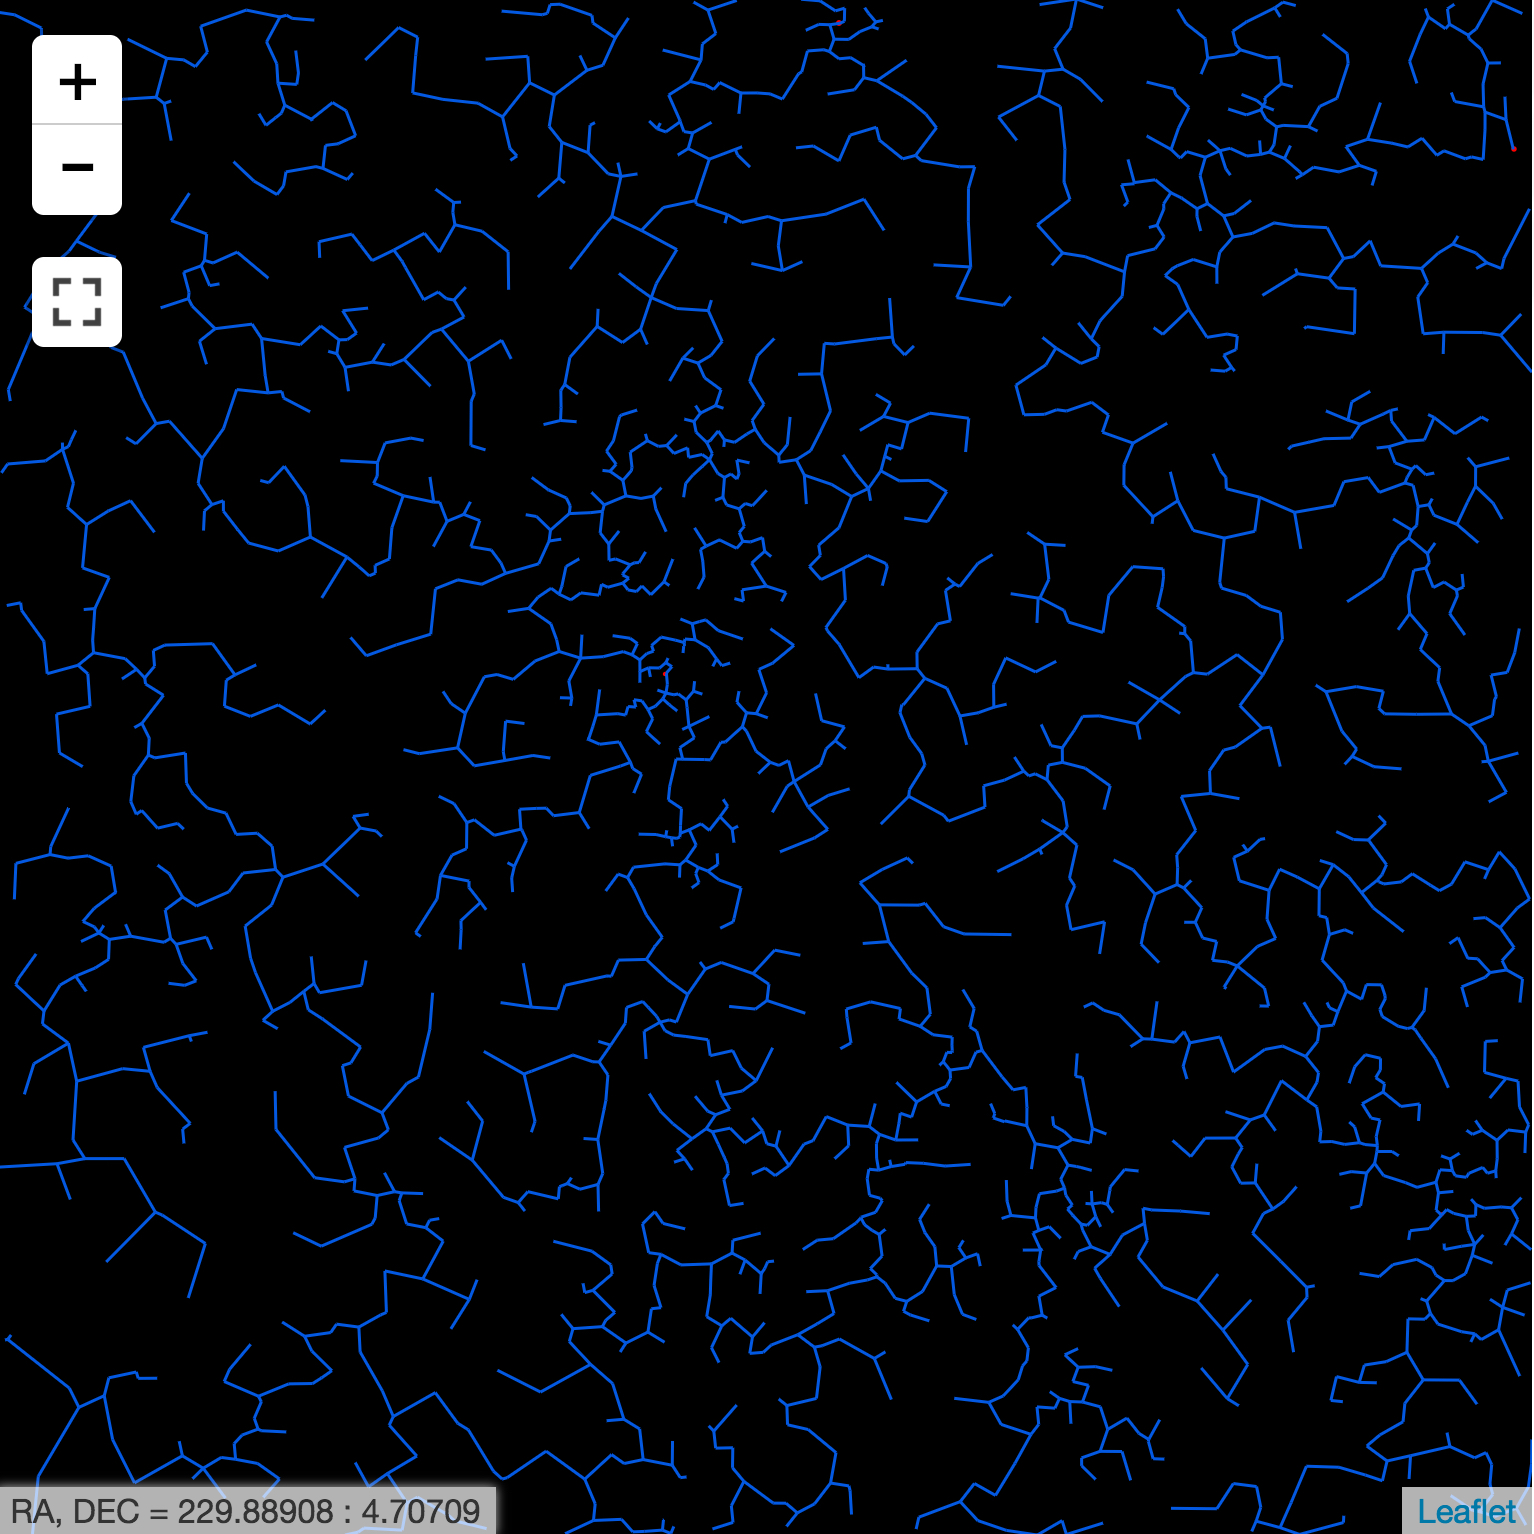
\includegraphics[width=0.4\textwidth]{FIG6b}\label{fig:m_2}}
\quad
\subfloat[Delaunay triangulation layer]{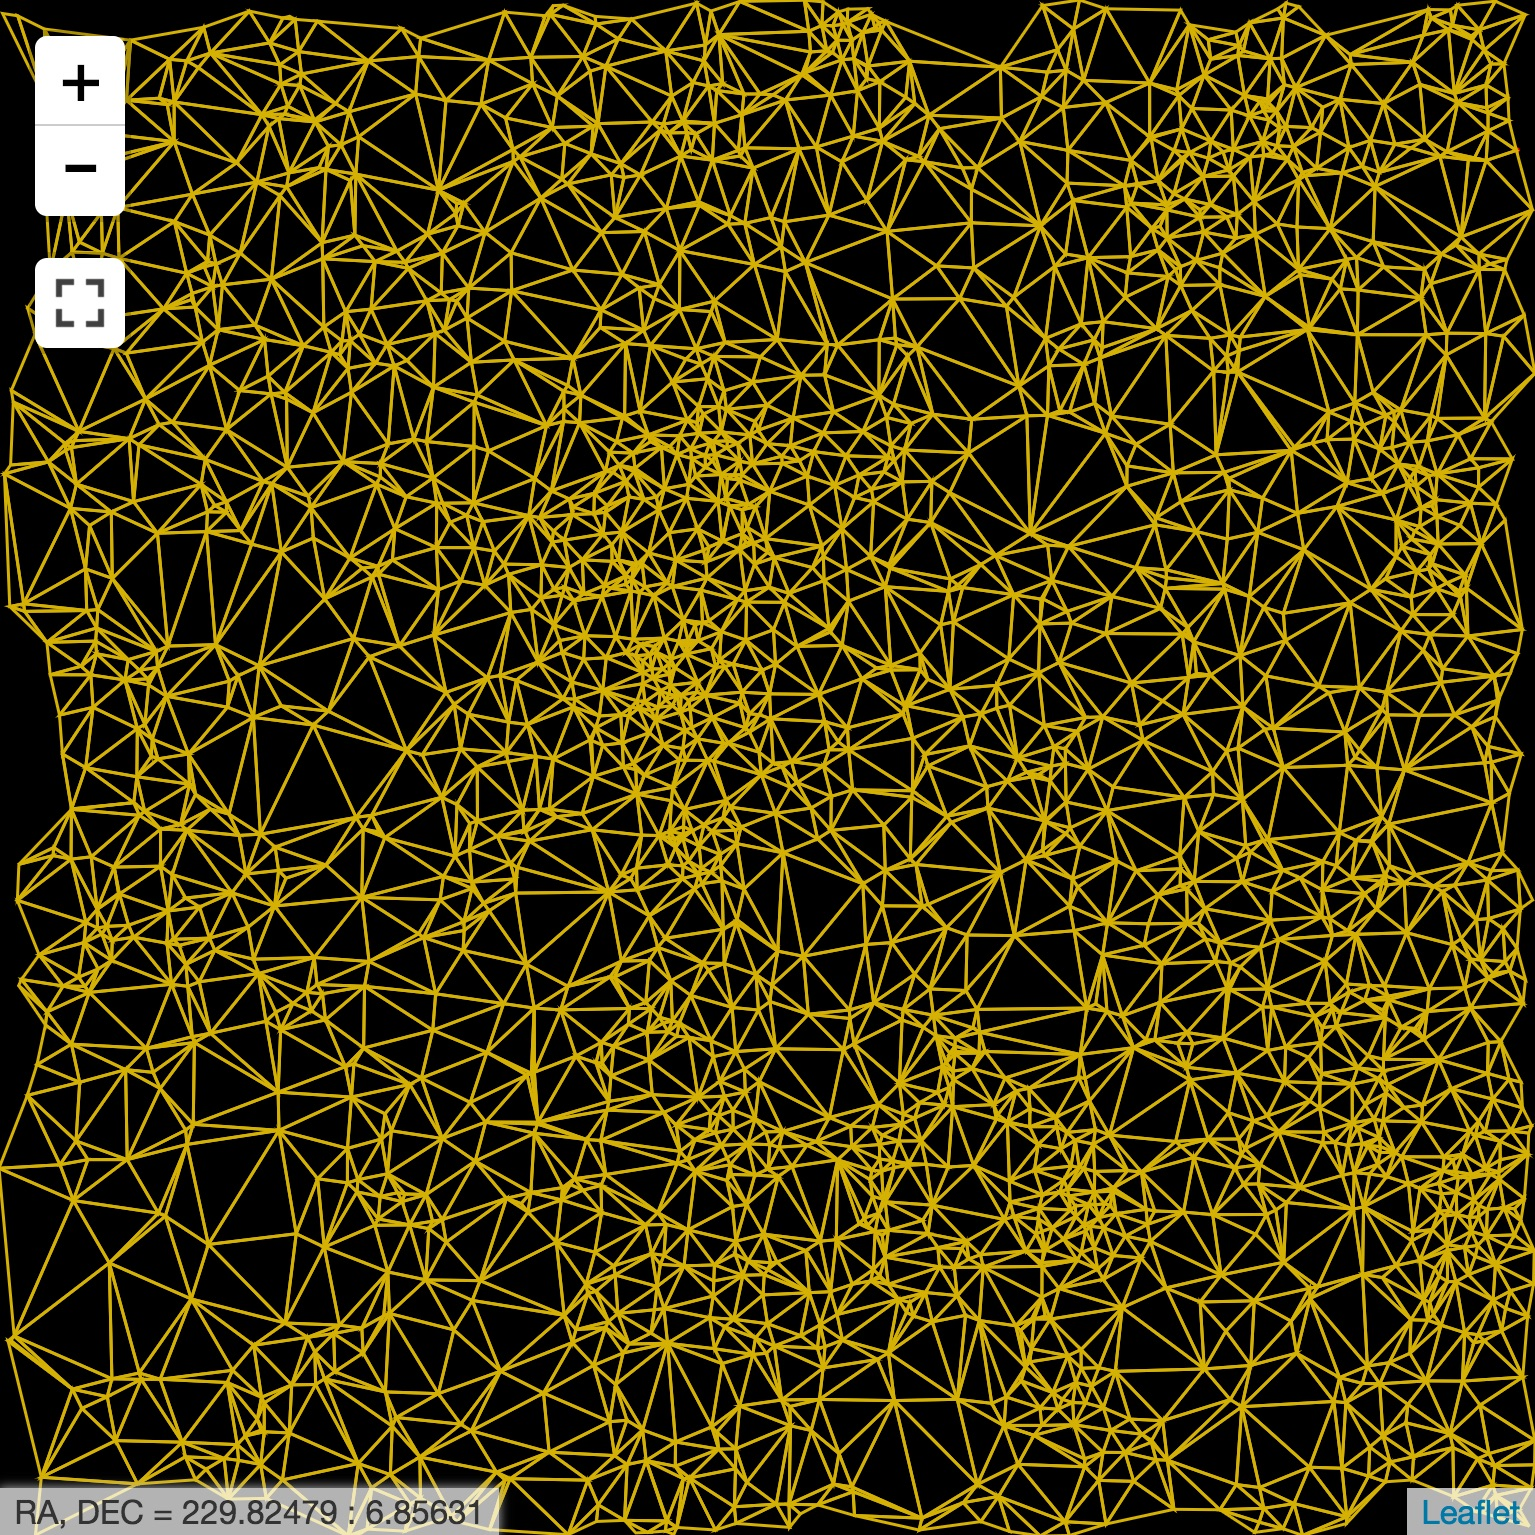
\includegraphics[width=0.4\textwidth]{FIG6c}\label{fig:d_3}}
\quad
\subfloat[HEALPix layer. This overlay is created with $nside=1024$ and zoomed in to level 4 for a clear view of the content.]{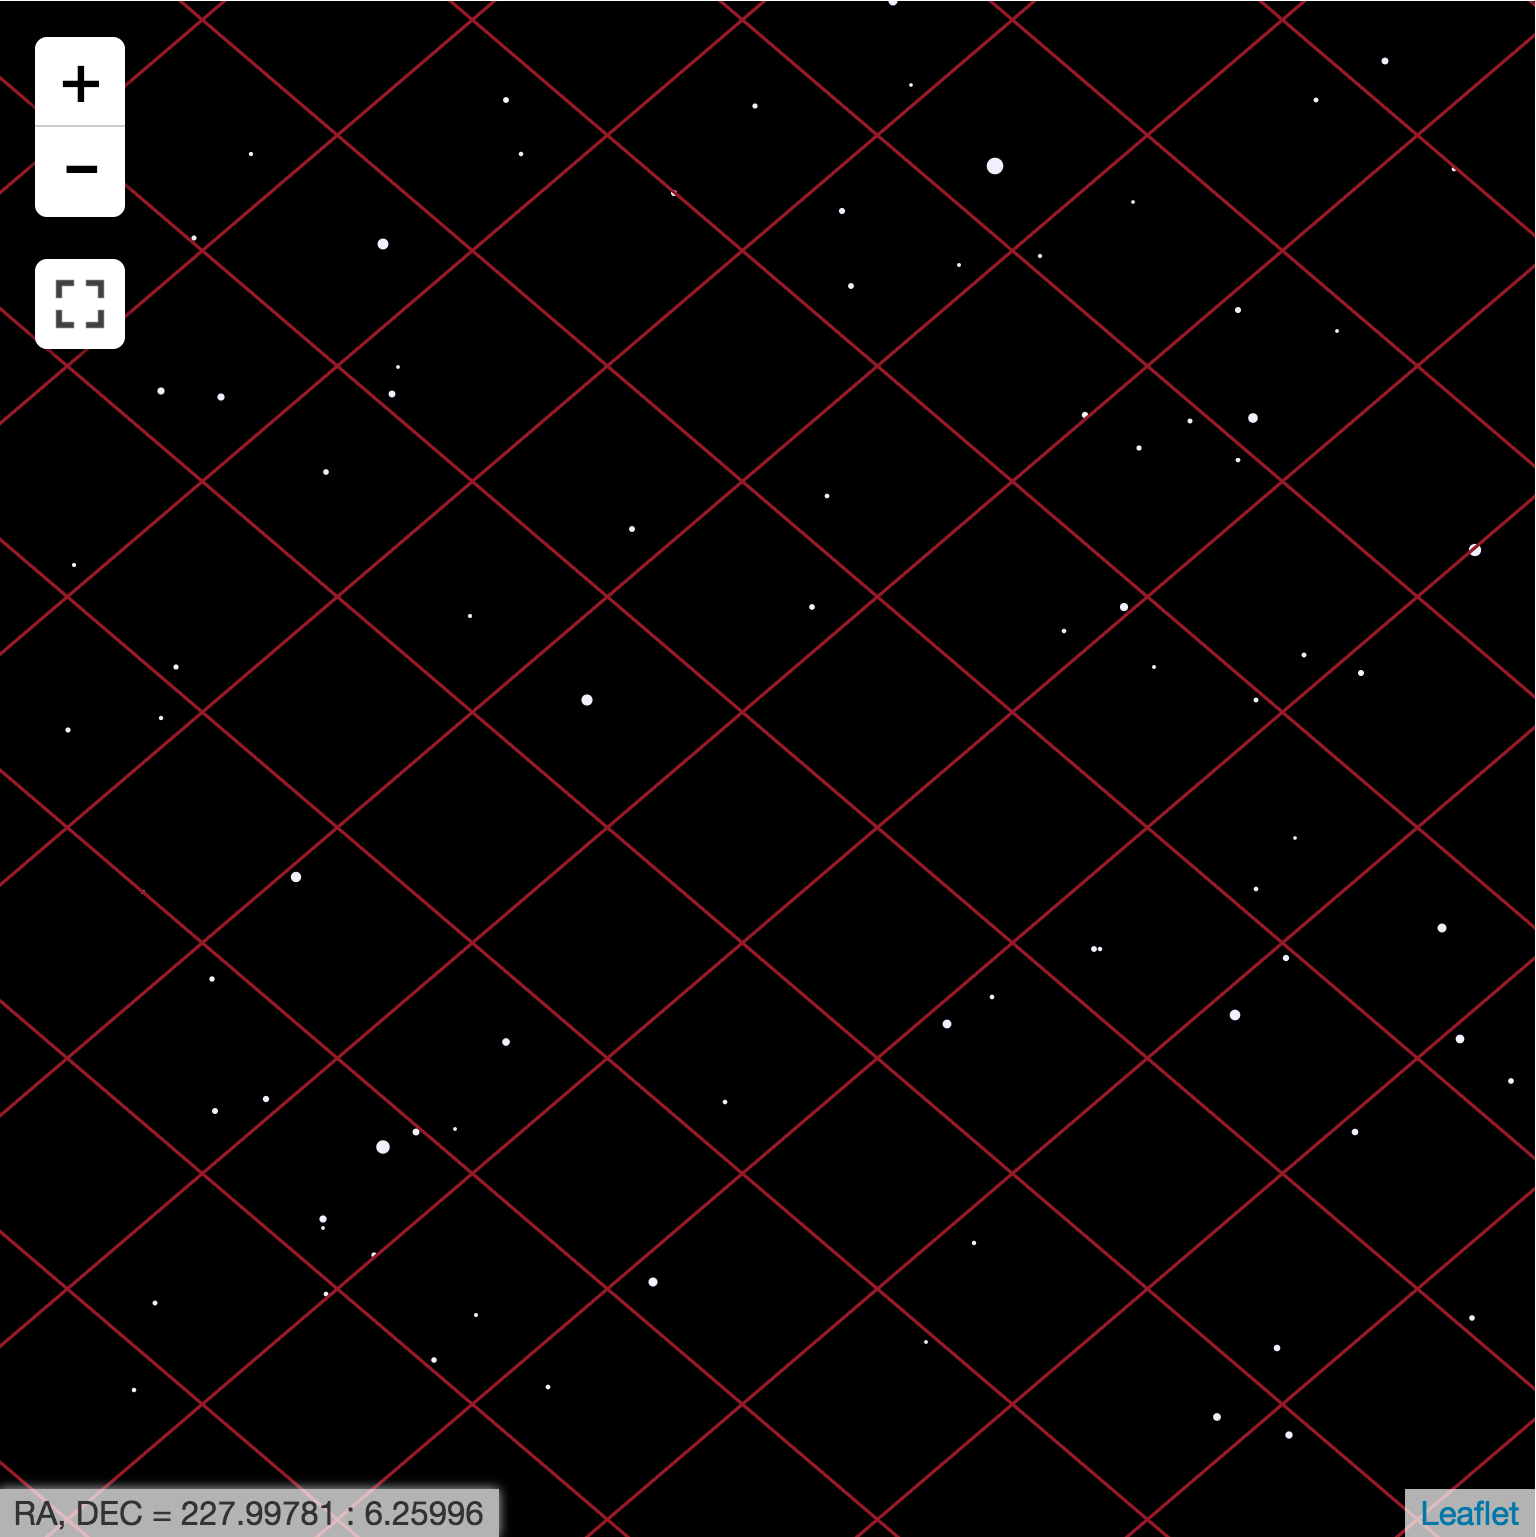
\includegraphics[width=0.4\textwidth]{FIG6d}\label{fig:h_4}}
\caption{Custom overlays appended on the same area of the sky, they can be over plotted on top of one another.}
\end{figure*}
\textit{Vizic} allows custom overlays to be appended on top of the tile-based layer.
\textit{Vizic} provides four pre-defined overlay layers, a Voronoi diagram \citep{Voronoi1908} layer, a Delaunay triangulation \citep{Delaunay} layer, a minimum spanning tree (MST) \citep{boruuvka1926, Kruskal1956} layer and a HEALPix\footnote{http://healpix.sourceforge.net} \citep{healpix} grid layer.
HEALPix stands for \textbf{H}ierarchical \textbf{E}qual \textbf{A}rea iso\textbf{L}atitude \textbf{Pix}elation.
These overlays are implemented through four different layer classes.
New layer widget can be added and removed from the map using the \texttt{add\_layer} function and the \texttt{remove\_layer} function of the \texttt{AstroMap} class respectively.
Once the overlay is added, it can scale and adapt itself to follow the interactive movements on the map. The rest of this subsection describes each overlay individually and briefly discusses its construction procedure.

\subsubsection{Voronoi Diagram Layer}
\label{voronoi}
A Voronoi diagram for $n$ given points (sites) in a plane divides up the plane into $n$ regions (Voronoi cells), such that each region contains only one site and for every point inside that region the associated site is always the closet site.
Each Voronoi cell is also a convex polygon. The shared side between any two polygons is the perpendicular bisector of the line segment connecting the two corresponding sites.
In astronomy, Voronoi diagram is commonly used in the study of cosmic structure \citep[e.g.,][]{voronoiLss, voronoiLss2, Weygaert2007}.
\textit{Vizic} generates the Voronoi diagram by treating astronomical sources as sites and computing the diagram based on their locations in the sky.

The Voronoi diagram overlay for a particular sky map can be created by initializing a \texttt{VoronoiLayer} object with the corresponding \texttt{GridLayer} object as the first argument.
Inside the \texttt{VoronoiLayer} initialization function, we first query the database for all objects on the given tiled catalog layer and convert their celestial coordinates into pixel coordinates on the screen following the projection mechanism described in Section \ref{basic}.
Then we compute the diagram for these objects and render the diagram by drawing the Voronoi cells using SVG polygons, which allows another level of customization such as color, width, etc.

\subsubsection{Delaunay Triangulation Layer}
We have also implemented a Delaunay triangulation overlay layer. The Delaunay triangulation for a set of points in a plane is a triangulation such that none of the points lies inside the circumcircles of the triangles in this triangulation.
A Delaunay triangulation can also be seen as the dual graph of the Voronoi diagram for the same set of points.
The Delaunay triangulation layer can be created using \texttt{DelaunayLayer} class. Similar to how we construct the Voronoi diagram overlay, we first project the given objects in a catalog onto the screen and calculate the Delaunay triangulation from the positions of these objects, finally we use SVG path elements to connect the vertices of each determined triangle.

\subsubsection{Minimum Spanning Tree Layer}
\label{mst}
In graph theory, a spanning tree of a connected and undirected graph is a tree that contains all the nodes in that graph.
If each edge in a given connected graph is assigned a weight, a MST of that graph is a spanning tree such that the total weight for all edges in this tree is the least.
In this overlay, we use astronomical objects as the nodes and assign each edge a weight equals to its length measured in degrees.

The minimum spanning tree is computed using a combination of packages in the SciPy Stack \citep{numpy, pandas, scipy, scikit-learn}. We first use \texttt{sklearn.neighbors} \citep{scikit-learn} to calculate the distance between each object and its nearest 20 (default value) neighbors and then determine the MST from all possible trees that can be created using the given edges \citep{scipy, Kruskal1956}.
The result is a compressed sparse matrix where the entry is zero if no edge exists between the two objects indexed by the row number and column number respectively.
By connecting the objects referred by each non-zero entries, we obtain the MST.

The minimum spanning tree overlay can be created by initiating a \texttt{MstLayer} object with the \texttt{GridLayer} object as the first argument.
Beyond visualizing the MST for a given set of objects on the sky map, we can also cut off the branches to select different structures \citep[e.g.,][]{Barrow1985,mst2}.
The user can prune the tree using the function \texttt{MstLayer.cut($r_{max}$, $n_{min}$)} with $r_{max}$ being the allowed maximum weight for saved edges and $n_{min}$ being the minimum number of edges that a saved sub branch must include.
As a result, only structures in a single branch with edges smaller than $r_{max}$ are kept.
% We can also specify the minimum number of vertices (sources) we want to display to help with the visualization of the structures.
Figure \ref{fig:mst_trimmed} shows a trimmed MST with a maximum weight of 0.055 degree or approximately 0.66 Mpc/h at a redshift (z) of 0.2 for groups with a minimum of eight members.

\begin{figure}[h]
  \centering
  %\textbf{Selection Tool}\par\medskip
  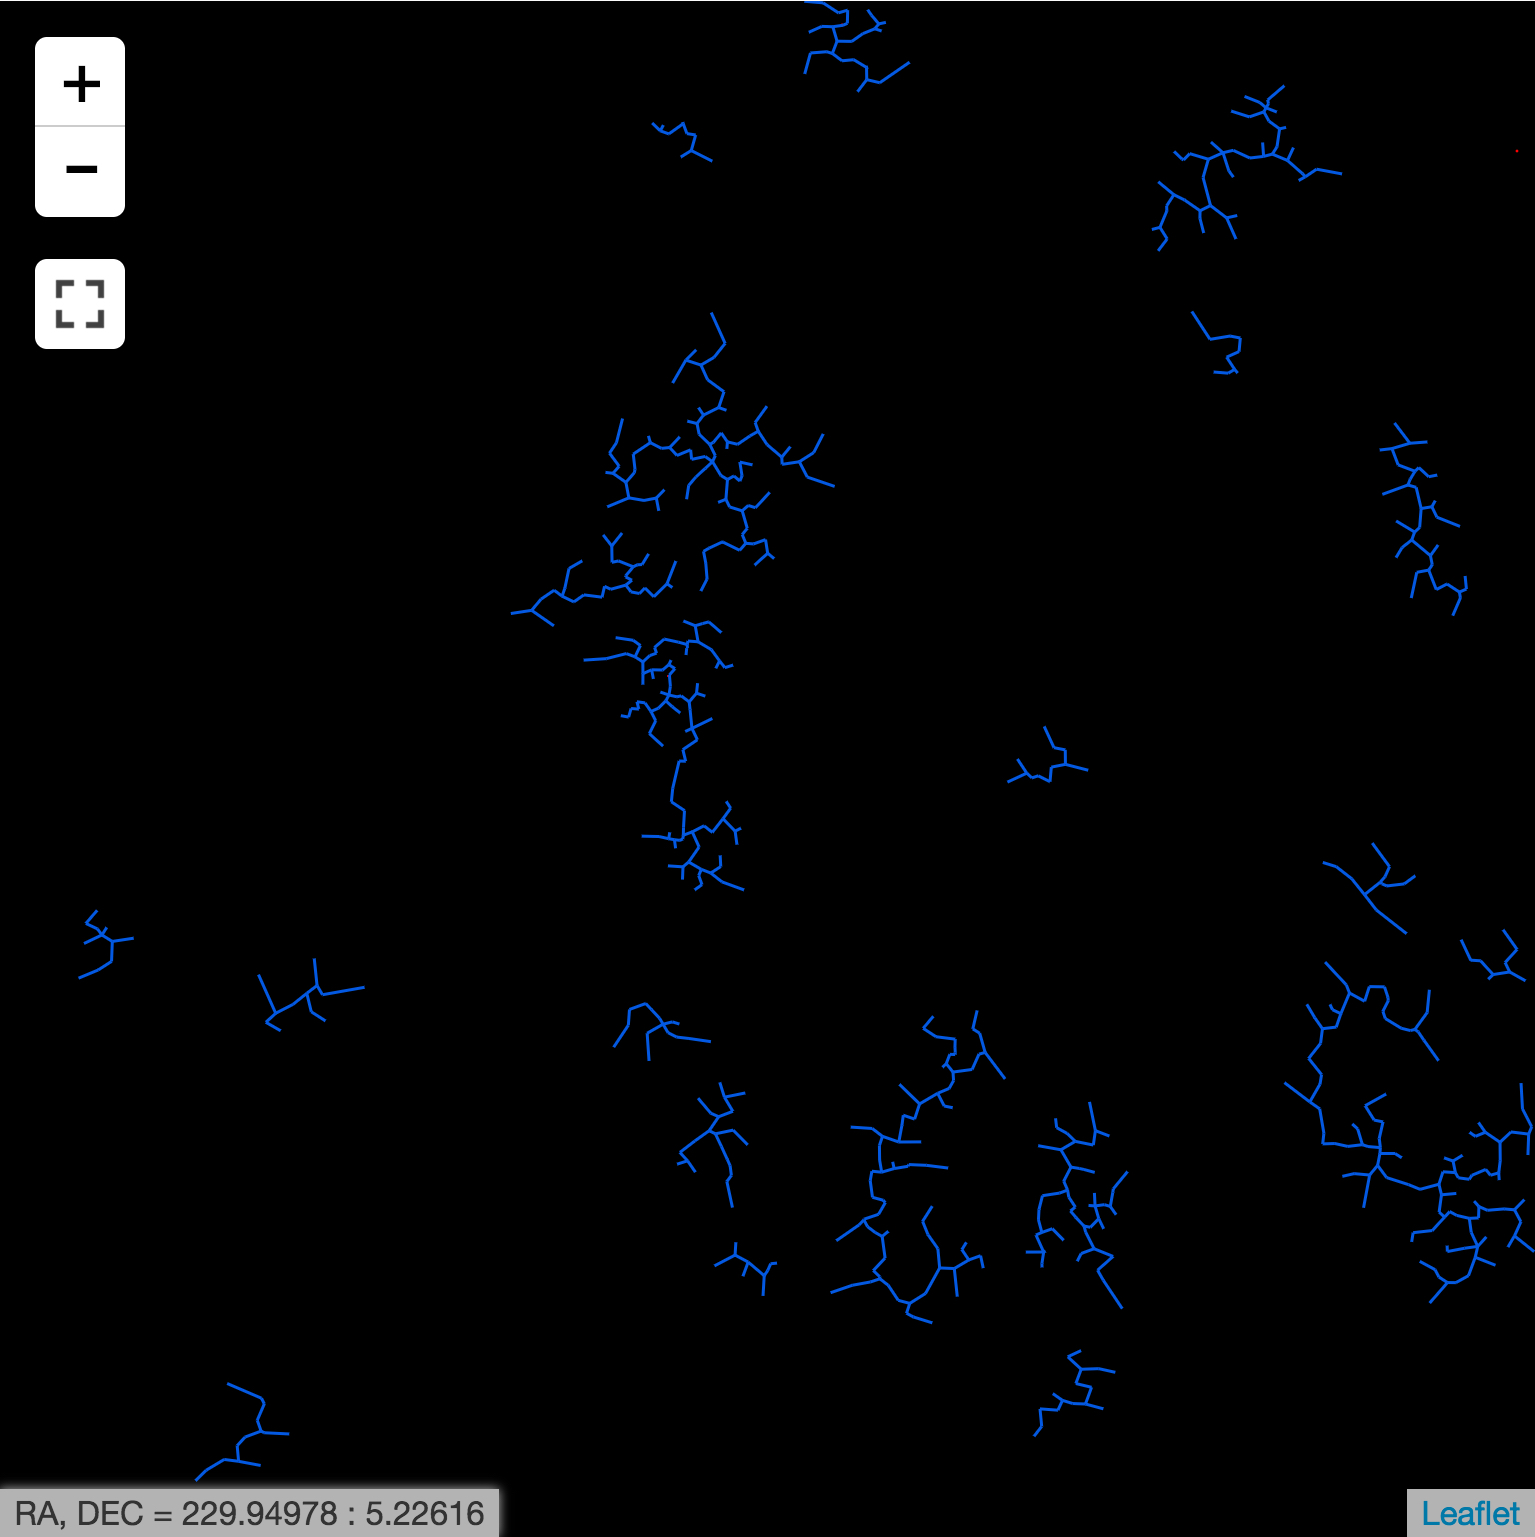
\includegraphics[width=0.43\textwidth]{FIG7}
  \caption{The tirmmed MST with $r_{max}=0.055^\circ$ (0.66 Mpc/h at z=0.2) and $n_{min}=8$}
  \label{fig:mst_trimmed}
\end{figure}

\subsubsection{HEALPix Grid Layer}
HEALPix is a method of pixelation that divides a spherical surface into quadrilaterals of equal area.
Each quadrilateral, in this case, is consider as a pixel. The lowest resolution of a HEALPix grid consist of 12 pixels and each higher resolution increase the total number pixels by four.
In our implementation, we use \textit{healpy}\footnote{https://github.com/healpy/healpy} to create the HEALPix grid, then project and connect the vertices of each pixel to draw the grid.
A demonstration of an appended HEALPix layer is shown in Figure \ref{fig:h_4}.

To display a HEALPix grid, a \texttt{HealpixLayer} object needs to be created first, with the \texttt{GridLayer} object of the target catalog layer as the first argument.
The resolution of the HEALPix grid can be specified by giving a new value to the keyword argument, \texttt{nside}, where the default is $1024$.
Like other overlay layers, a HEALPix grid overlay can be added or removed from the sky map using the \texttt{add\_layer} or \texttt{remove\_layer} function.
The advantage of using HEALPix grid is that we can then easily compute densities or other quantities per HEALPix pixel, which will improve the interaction with the datasets further allowing extra types of density based analysis.
\end{document}
